\chapter{Rendering Our First Triangle}

\begin{figure}[ht]
    \centering
    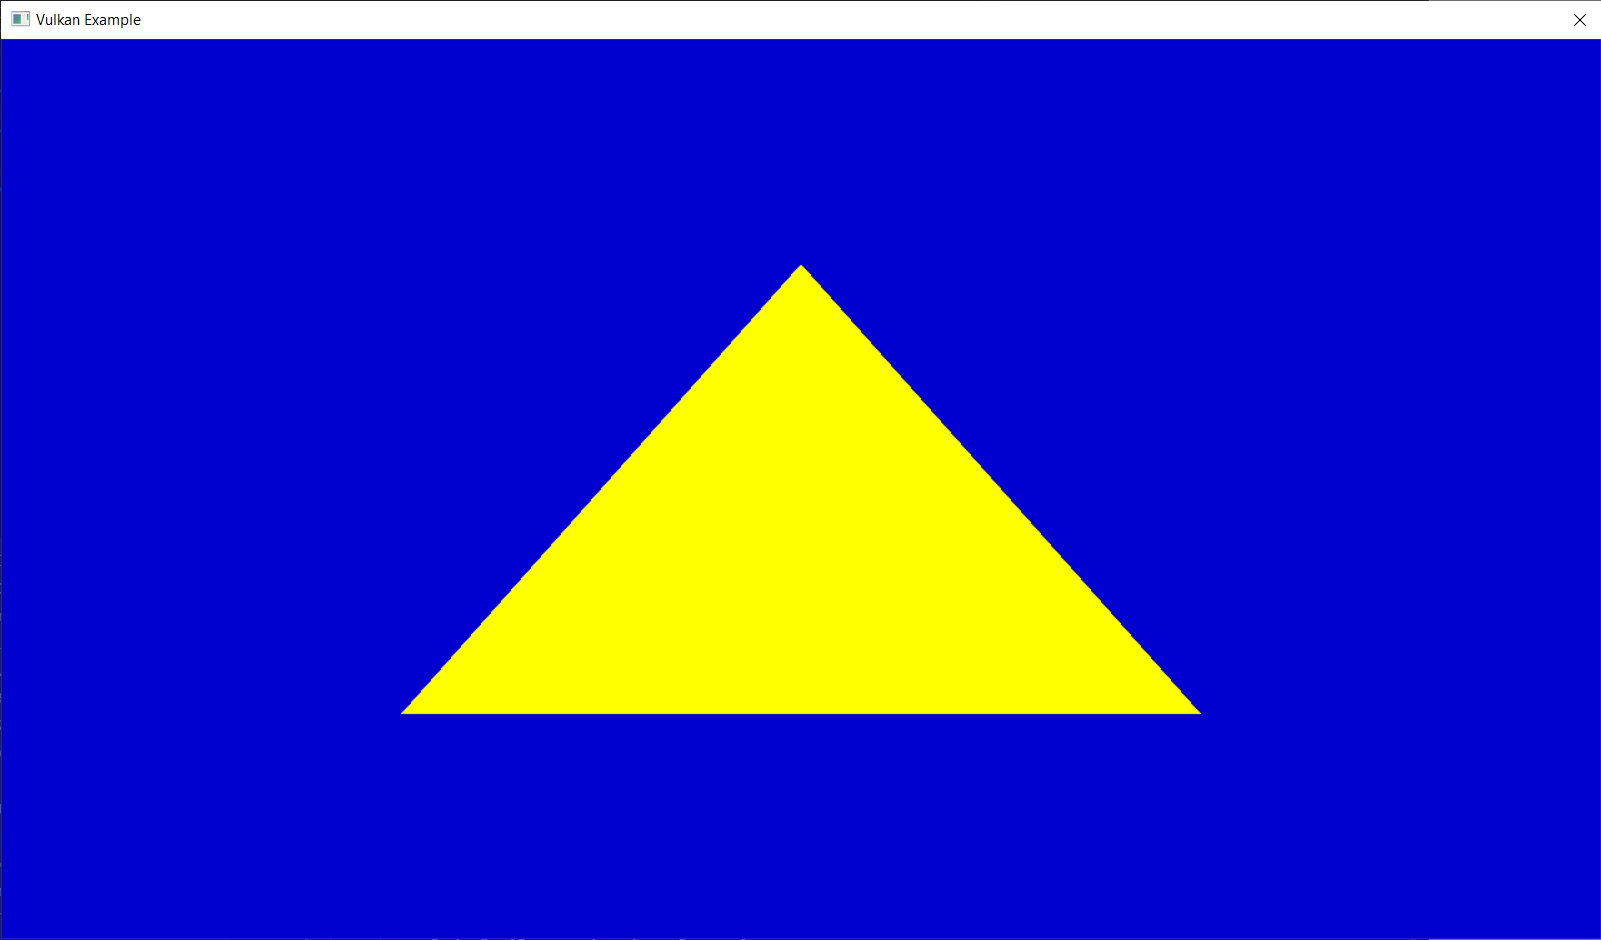
\includegraphics[scale=0.20]{images/ChTriangle/Triangle.png}
    \caption{Rendering our triangle}
    \label{fig::RenderTriangle}
\end{figure}

In this chapter we see how to render a triangle on the screen.
If we are able to draw a single triangle, then we can draw almost any shape.
We can do this by considering the shape we want to draw as if it were
made up of one or more triangles and then drawing them.

In order to render a triangle using Vulkan, we have to set up a pipeline state
object.
This object describes the entire state of our pipeline.
Thus, it also describes how we want to draw something.

In our application main loop, during our command buffer recording, we then
simply need to use our pipeline state object and issue a draw call that activates
our pipeline and draws what we want.

\section{Create A Pipeline State Object}

To create a pipeline state object we use \texttt{vkCreateGraphicsPipelines}.

\begin{minipage}{\linewidth}{\noindent}
    \lstinputlisting[
        language=C++,
        caption={Create a pipeline state object},
        label={lst::CreatePipelineStateObject}
        ]{src/ChTriangle/CreatePipelineStateObject.cpp}
\end{minipage}

\subsection{VkGraphicsPipelineCreateInfo}

We use a \texttt{VkGraphicsPipelineCreateInfo} struct to configure the pipeline state
object we are about to create.

\texttt{layout} is the description of binding locations used by both the pipeline
and descriptor sets used with the pipeline.
It doesn't matter in our case.
We will see its use when we talk about uniforms.

\texttt{renderPass} is a handle to a render pass object describing the environment
in which the pipeline will be used.

\texttt{subpass} is the index of the subpass in the render pass where
this pipeline will be used.

We will explain the meaning of the remaining relevant struct fields
in the next sections.

\begin{minipage}{\linewidth}{\noindent}
    \lstinputlisting[
        language=C++,
        caption={Configure pipeline state object},
        label={lst::VkGraphicsPipelineCreateInfo}
        ]{src/ChTriangle/VkGraphicsPipelineCreateInfo.cpp}
\end{minipage}

\subsection{Shader Stages}

We have to specify a collection of all shader stages and shader programs that
will be used during rendering.

\begin{minipage}{\linewidth}{\noindent}
    \lstinputlisting[
        language=C++,
        caption={Shader stages},
        label={lst::ShaderStages}
        ]{src/ChTriangle/ShaderStages.cpp}
\end{minipage}

\subsubsection{VkPipelineShaderStageCreateInfo}

In our case we need two instances of a \texttt{VkPipelineShaderStageCreateInfo}
struct that describe our vertex and our fragment shader stages.

\texttt{stage} is a \texttt{VkShaderStageFlagBits} value specifying the
pipeline stage.
\texttt{module} is a shader module object containing the shader for this stage.
\texttt{pName} is a string specifying the entry point name of the shader for this
stage.

\begin{minipage}{\linewidth}{\noindent}
    \lstinputlisting[
        language=C++,
        caption={Describe a shader stage},
        label={lst::VkPipelineShaderStageCreateInfo}
        ]{src/ChTriangle/VkPipelineShaderStageCreateInfo.cpp}
\end{minipage}

In order to create our vertex shader stage we need to pass the shader module
that contains our vertex shader code and use the
\texttt{VK\_SHADER\_STAGE\_VERTEX\_BIT} stage flag bit.

In order to create our fragment shader stage we need to pass the shader module
that contains our fragment shader code and use the
\mbox{\texttt{VK\_SHADER\_STAGE\_FRAGMENT\_BIT}} stage flag bit.

\subsubsection{VkShaderModule}

To create a shader module we need to load our shader code written
in SPIR-V binary format.
Then, we simply use \texttt{vkCreateShaderModule}.
After creating our shader module, we can discard our loaded shader code.

\begin{minipage}{\linewidth}{\noindent}
    \lstinputlisting[
        language=C++,
        caption={Create a shader module},
        label={lst::VkShaderModule}
        ]{src/ChTriangle/VkShaderModule.cpp}
\end{minipage}

In our case, we create one shader module for our vertex shader and one shader
module for our fragment shader.

\subsubsection{Vertex Shader Code}

We write our vertex shader in GLSL.
We use a \texttt{.vert} file extension.
The built in \texttt{gl\_VertexIndex} variable contains the index of the
current vertex.
This is usually an index into the vertex buffer, but in our case
it will be an index into an hardcoded array of vertex data.
We will see how to upload vertex data later.
The built in variable \texttt{gl\_Position} functions as the output.

\begin{minipage}{\linewidth}{\noindent}
    \lstinputlisting[
        language=C++,
        caption={Our first vertex shader},
        label={lst::FirstVertexShader}
        ]{src/ChTriangle/shader.vert}
\end{minipage}

\subsubsection{Fragment Shader Code}

We write our fragment shader in GLSL.
We use a \texttt{.frag} file extension.
Unlike \texttt{gl\_Position} in the vertex shader, there is no built in
variable to output a color for the current fragment.
We have to specify our own output variable.
The color yellow is written to this \texttt{outColor} variable.

\begin{minipage}{\linewidth}{\noindent}
    \lstinputlisting[
        language=C++,
        caption={Our first fragment shader},
        label={lst::FirstFragmentShader}
        ]{src/ChTriangle/shader.frag}
\end{minipage}

\subsubsection{Compiling GLSL To SPIR-V}

Since we write our shaders in GLSL, we
need to compile them into SPIR-V binary format.
The compiler that does this is shipped together with the Vulkan SDK.

\subsubsection{Cleanup}

After the pipeline state object is created, we can destroy the shader modules
we created using \texttt{vkDestroyShaderModule}.

\subsection{Vertex Input State}

We use a \texttt{VkPipelineVertexInputStateCreateInfo} struct to configure the
vertex input state of the pipeline object we are about to create.

This struct describes the format of the vertex data that will be passed
to the vertex shader.
Here we don't have any vertex data.

\begin{minipage}{\linewidth}{\noindent}
    \lstinputlisting[
        language=C++,
        caption={Configure vertex input state},
        label={lst::EmptyVertexInputState}
        ]{src/ChTriangle/VertexInputState.cpp}
\end{minipage}

\subsection{Input Assembly State}

We use a \texttt{VkPipelineInputAssemblyStateCreateInfo} struct to configure the
input assembly state of the pipeline object we are about to create.

This struct describes how vertices are assembled into primitives.
In our case, the vertex data we have hardcoded into our vertex shader specifies
a list of triangles.

\begin{minipage}{\linewidth}{\noindent}
    \lstinputlisting[
        language=C++,
        caption={Configure input assembly state},
        label={lst::VkPipelineInputAssemblyStateCreateInfo}
        ]{src/ChTriangle/VkPipelineInputAssemblyStateCreateInfo.cpp}
\end{minipage}

\subsection{Viewport State}

We use a \texttt{VkPipelineViewportStateCreateInfo} struct to configure
the viewport state of the pipeline object we are about to create.

\begin{minipage}{\linewidth}{\noindent}
    \lstinputlisting[
        language=C++,
        caption={Configure viewport state},
        label={lst::VkPipelineViewportStateCreateInfo}
        ]{src/ChTriangle/VkPipelineViewportStateCreateInfo.cpp}
\end{minipage}

\subsubsection{Viewports}

The \texttt{pViewports} struct field
is an array of viewports that will be used by our pipeline.
A viewport describes what part of the image (or texture, or window) we want to draw.
In our case we want to draw the entire image.
The graphics pipeline also uses viewports to transform normalized device
coordinates into screen coordinates.

\begin{minipage}{\linewidth}{\noindent}
    \lstinputlisting[
        language=C++,
        caption={Viewport},
        label={lst::Viewport}
        ]{src/ChTriangle/Viewport.cpp}
\end{minipage}

\subsubsection{Scissors}

The \texttt{pScissors} struct field
is an array of scissor rectangles.
The graphics pipeline uses these rectangles to decide which fragments to discard.
Any pixels outside the scissor rectangles will be discarded by the rasterizer.
In our case we don't discard any fragments.

\begin{minipage}{\linewidth}{\noindent}
    \lstinputlisting[
        language=C++,
        caption={Scissor},
        label={lst::Scissor}
        ]{src/ChTriangle/Scissor.cpp}
\end{minipage}

\subsection{Rasterization State}

We use a \texttt{VkPipelineRasterizationStateCreateInfo} struct to configure
the rasterization state of the pipeline object we are about to create.

This struct describes how polygons are going to be rasterized
(changed into fragments).
The rasterizer takes the geometry that is shaped by the vertices from the
vertex shader and turns it into fragments to be colored by the fragment shader.
The rasterizer also performs depth testing, face culling and the scissor test.

\texttt{polygonMode} determines how fragments are generated for geometry.
Using any mode other than fill requires enabling a GPU feature.
\texttt{lineWidth} describes the width of rasterized line segments.

\begin{minipage}{\linewidth}{\noindent}
    \lstinputlisting[
        language=C++,
        caption={Rasterization state},
        label={lst::VkPipelineRasterizationStateCreateInfo}
        ]{src/ChTriangle/VkPipelineRasterizationStateCreateInfo.cpp}
\end{minipage}

\subsection{Multisample State}

We use a \texttt{VkPipelineMultisampleStateCreateInfo} struct to configure
the multisample state of the pipeline object we are about to create.
We don't use multisampling here.

\begin{minipage}{\linewidth}{\noindent}
    \lstinputlisting[
        language=C++,
        caption={Multisample state},
        label={lst::VkPipelineMultisampleStateCreateInfo}
        ]{src/ChTriangle/VkPipelineMultisampleStateCreateInfo.cpp}
\end{minipage}

\subsection{Depth Stencil State}

We use a \texttt{VkPipelineDepthStencilStateCreateInfo} struct to configure
the depth stencil state of the pipeline object we are about to create.
We neither use depth testing nor stencil testing here.

\begin{minipage}{\linewidth}{\noindent}
    \lstinputlisting[
        language=C++,
        caption={Depth stencil state},
        label={lst::VkPipelineDepthStencilStateCreateInfo}
        ]{src/ChTriangle/VkPipelineDepthStencilStateCreateInfo.cpp}
\end{minipage}

\subsection{Color Blend State}

We use a \texttt{VkPipelineColorBlendStateCreateInfo} struct to configure
the color blend state of the pipeline object we are about to create.

After a fragment shader has returned a color,
it needs to be combined with the color that is already in the framebuffer.
This transformation is known as color blending.

\texttt{pAttachments} is an array of of
\texttt{VkPipelineColorBlendAttachmentState} structures defining blend state for
each color attachment.

\begin{minipage}{\linewidth}{\noindent}
    \lstinputlisting[
        language=C++,
        caption={Color blend state},
        label={lst::VkPipelineColorBlendStateCreateInfo}
        ]{src/ChTriangle/VkPipelineColorBlendStateCreateInfo.cpp}
\end{minipage}

\subsubsection{VkPipelineColorBlendAttachmentState}

We have to configure how color blending works for every color attachment
in our framebuffer.
Since we have only one color attachment, we need only one description.

\texttt{blendEnable} controls whether blending is enabled for the corresponding
color attachment.
If blending is not enabled, the source fragment's color for that attachment
is passed through unmodified.

\texttt{colorWriteMask} is a bitmask specifying which of the R, G, B, and/or A
components are enabled for writing.
This bitmask determines whether the final color values R, G, B and A are written
to the framebuffer attachment.

In our case, we don't use color blending.
We simply write all the color components to the framebuffer as they are.

\begin{minipage}{\linewidth}{\noindent}
    \lstinputlisting[
        language=C++,
        caption={Color blend attachment state},
        label={lst::VkPipelineColorBlendAttachmentState}
        ]{src/ChTriangle/VkPipelineColorBlendAttachmentState.cpp}
\end{minipage}

\subsection{Pipeline Layout}

Before creating our pipeline, we need to define its layout.
We do this by creating a pipeline layout object.

\begin{minipage}{\linewidth}{\noindent}
    \lstinputlisting[
        language=C++,
        caption={Create our pipeline layour},
        label={lst::CreatePipelineLayout}
        ]{src/ChTriangle/CreatePipelineLayout.cpp}
\end{minipage}

\subsubsection{VkPipelineLayoutCreateInfo}

We use a \texttt{VkPipelineLayoutCreateInfo} struct to configure the pipeline
layout we are about to create.
In this scenario we can ignore our pipeline layout.
We will use it in later chapters.

\begin{minipage}{\linewidth}{\noindent}
    \lstinputlisting[
        language=C++,
        caption={Configure our pipeline layout},
        label={lst::VkPipelineLayoutCreateInfo}
        ]{src/ChTriangle/VkPipelineLayoutCreateInfo.cpp}
\end{minipage}

\subsection{Cleanup}

We first destroy our pipeline state object using \texttt{vkDestroyPipeline}.
Then, we destroy our pipeline layout using \texttt{vkDestroyPipelineLayout}.

\section{Use Our Pipeline To Draw A Triangle}

Now that we have created our pipeline state object we can use it
to set the graphics pipeline current state.
Then we can tell our graphics pipeline to draw three vertices.
This will lead to our triangle being rendered.

\begin{minipage}{\linewidth}{\noindent}
    \lstinputlisting[
        language=C++,
        caption={Rendering our triangle},
        label={lst::RenderTriangle}
        ]{src/ChTriangle/RenderTriangle.cpp}
\end{minipage}
